\documentclass[12pt]{article}
\usepackage[utf8]{inputenc}
\usepackage[T1]{fontenc}
\usepackage{geometry}
\usepackage{graphicx}
\usepackage{makeidx}
\geometry{margin=2.5cm}

\begin{document}
	
	\thispagestyle{empty}
	
	\begin{center}
		\includegraphics[width=3.1cm,height=2cm]{logo}\\
		UNIVERSIDAD SIMÓN BOLÍVAR\\
		DEPARTAMENTO DE ELECTRÓNICA Y CIRCUITOS\\
		EC1281 - LABORATORIO DE MEDICIONES ELÉCTRICAS\\
		SECCIÓN 1 - GRUPO 1\\
		
		\vspace{7cm}
		\textbf{\Large INFORME - PRÁCTICA \#}\\
		INTRODUCCIÓN AL LABORATORIO\\
	\end{center}
	
	\begin{flushleft}
		\vspace{9cm}
		\hfill Integrantes:\\
		\hfill {\large Luis Becerra - 1910557}\\
		\hfill {\large Lorena Rojas - 1910469}\\
	\end{flushleft}
	
	\newpage
	
	\pagenumbering{roman}
	
	\begin{center}
		\textbf{\large RESUMEN}\\
	\end{center}
	
	Inserte resumen
	
	\newpage
	
	\begin{center}
		\textbf{\large ÍNDICE}\\
	\end{center}
	
	\noindent \textbf{RESUMEN} \hfill \textbf{I}\\
	\noindent \textbf{ÍNDICE} \hfill \textbf{II}\\
	\noindent \textbf{MARCO TEÓRICO} \hfill \textbf{1}\\
	\noindent \textbf{METEDOLOGÍA} \hfill \textbf{4}\\
	\noindent \textbf{RESULTADOS} \hfill \textbf{5}\\
	\noindent \textbf{ANÁLISIS DE RESULTADOS} \hfill \textbf{13}\\
	\noindent \textbf{CONCLUSIONES} \hfill \textbf{14}\\
	\noindent \textbf{BIBLIOGRAFÍA} \hfill \textbf{15}\\
	\noindent \textbf{ANEXOS} \hfill \textbf{16}\\
	
	\newpage
	
	\pagenumbering{arabic}
	
	\begin{center}
		\textbf{\large MARCO TEÓRICO}\\
	\end{center}
	
	\textbf{1. }\\
	
	Inserte inciso 1
	
	\begin{itemize}
		\item \textbf{Sub-elemento 1 del inciso } inserte lo que corresponda
		
	\end{itemize}

	\newpage
	
	\begin{center}
		\textbf{\large METODOLOGÍA}\\
	\end{center}
	
	Inserte metodología
	
	\newpage
	
	\begin{center}
		\textbf{\large RESULTADOS}\\
	\end{center}
	
	\noindent En el laboratorio se midió lo siguiente:
	
	\begin{center}
		\includegraphics[width=16cm,height=20cm]{Img/anex_lab_4_0001}
	\end{center}
	
	\begin{center}
		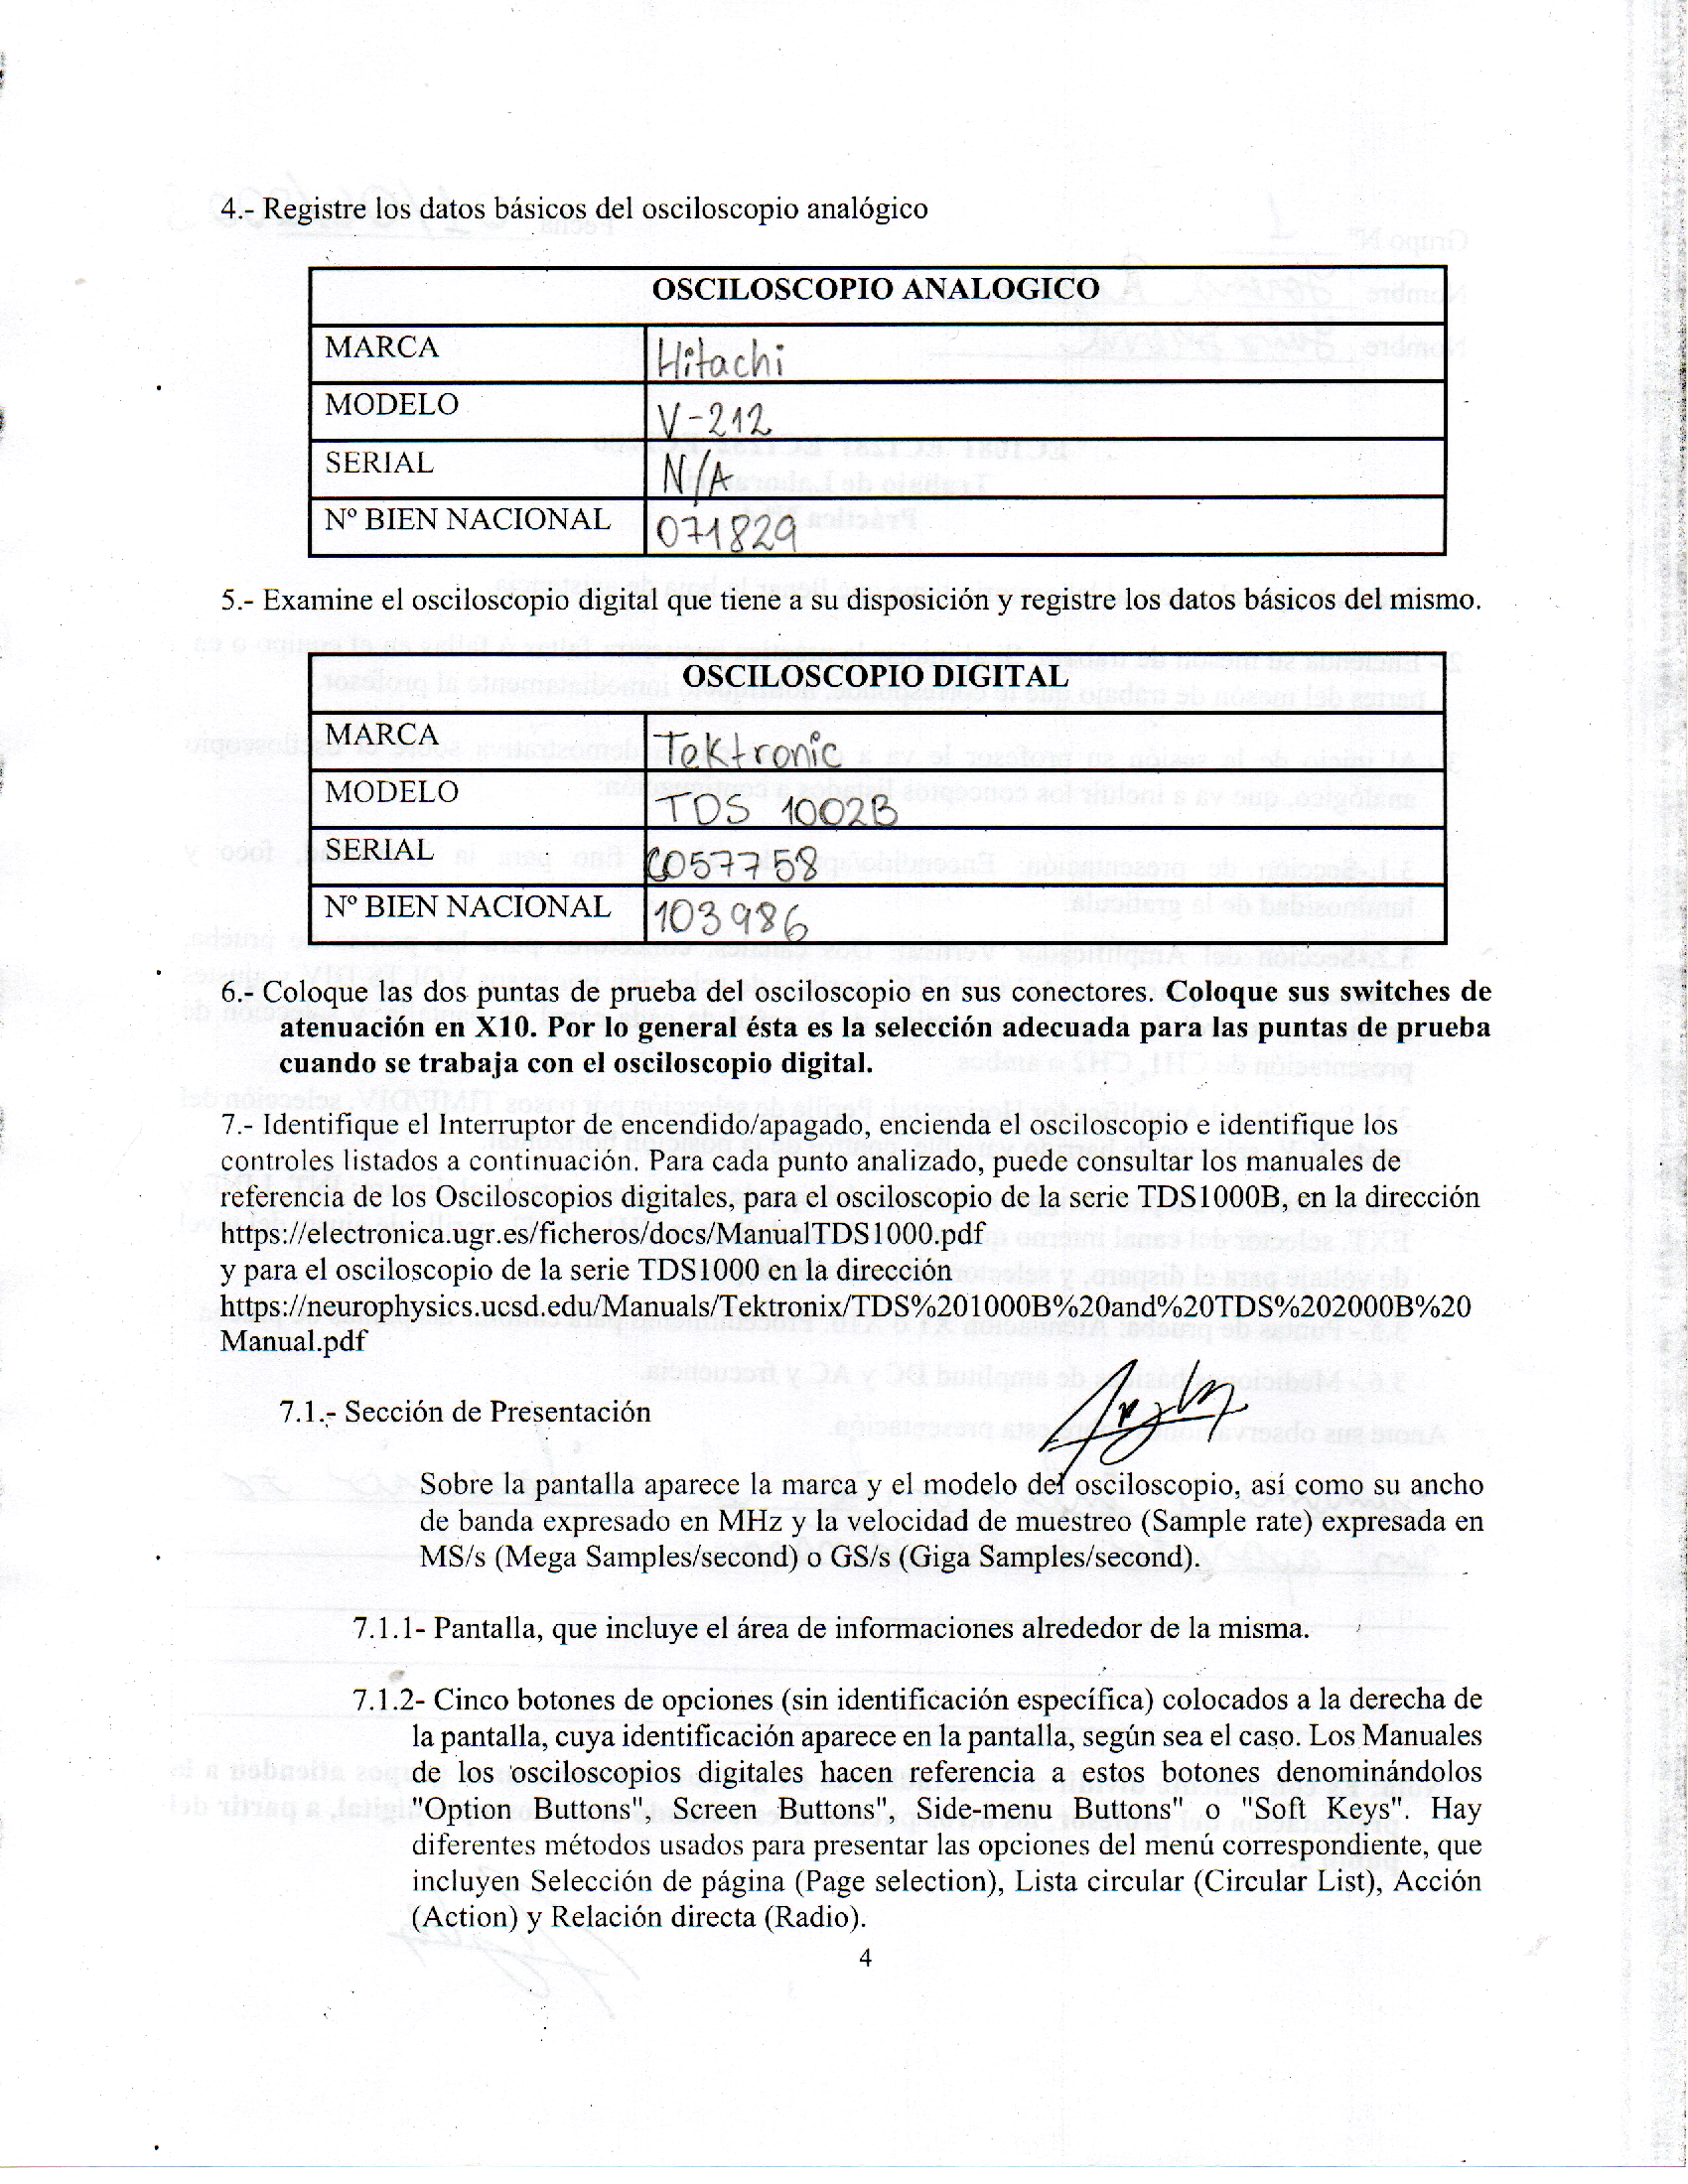
\includegraphics[width=16cm,height=20cm]{Img/anex_lab_4_0002}
	\end{center}
	
	\begin{center}
		\includegraphics[width=16cm,height=20cm]{Img/anex_lab_4_0003}
	\end{center}
	
	\begin{center}
		\includegraphics[width=16cm,height=20cm]{Img/anex_lab_4_0004}
	\end{center}
	
	\begin{center}
		\includegraphics[width=16cm,height=20cm]{Img/anex_lab_4_0005}
	\end{center}
	
	\begin{center}
		\includegraphics[width=16cm,height=20cm]{Img/anex_lab_4_0006}
	\end{center}
	
	\begin{center}
		\includegraphics[width=16cm,height=20cm]{Img/anex_lab_4_0007}
	\end{center}
	
	
	\newpage
	
	\newpage
	
	\begin{center}
		\textbf{\large ANÁLISIS DE RESULTADOS}\\
	\end{center}
	
	\noindent Tiempo atrás durante la práctica de Spice, uno de los circuitos simulados concuerda con el que se estudió durante esta práctica, un circuito RC en corriente alterna, el circuito en cuestión seguía el siguiente esquema:
	
	\begin{center}
		\includegraphics[width=10cm,height=8cm]{Img/ac_rc}
	\end{center}
	
	\noindent Al medir el voltaje de la fuente y en el capacitor para esa disposición se obtuvo el siguiente análisis:
	
	\begin{center}
		\includegraphics[width=10cm,height=8cm]{Img/fuente_capacitor_spice}
	\end{center}
	
	\newpage
	
	\noindent Luego al replicar ese circuito en el laboratorio se obtuvo:
	
	\begin{center}
		\includegraphics[width=10cm,height=8cm]{Img/fuente_capacitor}
	\end{center}
	
	\noindent Se puede apreciar que el defase del capacitor respecto a la fuente se mantiene igual como debería y que ambas gráficas son sumamente similares, las diferencias radican en detalles como la salida en el generador de ondas y la escala observada, sin embargo, las gráficas son perfectamente análogas.
	
	\noindent También tendremos que al medir el voltaje en la resistencia vs el voltaje en el capacitor en spice resultó en:
	
	\begin{center}
		\includegraphics[width=10cm,height=8cm]{Img/capacitor_resistencia_spice}
	\end{center}
	
	\noindent En spice cambiar los elementos evaluados sólo implicaba, sin embargo en la práctica implicó cambiar las conexiones del osciloscopio e invertir la señal del capacitor ya que al ser medida por algunas carracterísticas del modo flotante, el voltaje medido en el capacitor tenía polaridad invertida, después de configurar todo, se obtuvo:
	
	\begin{center}
		\includegraphics[width=10cm,height=8cm]{Img/capacitor_resistencia}
	\end{center}

	\noindent Como se puede apreciar, al igual que antes, la gráfica obtenida es análoga a la ue generó spice, confirmando así que lo planteado teóricamente se cumple al tener un circuito físico funcionando.\\
	
	\noindent Para ambos pares de gráficas destaca que cada par es análogo entre sí y ue las diferencias radican en las escalas del multímetro, el voltaje suministrado por el generador de fuentes y la configuracipon de la gráfica en spice, aún así, queda en evidencia que spice es una herramienta formidable para probar circuito antes de montarlos, lo que permite esstimar eficiencia, optimizar gastos y perfeccionar los circuitos.
	
	\newpage
	
	\begin{center}
		\textbf{\large CONCLUSIONES}\\
	\end{center}
	
	\renewcommand{\theenumi}{\alph{enumi}} %Letras minúsculas 
	
	\begin{enumerate}
		
		\item Precisión y exactitud de las medidas de voltaje DC
		tomadas con el osciloscopio:
		
		\noindent En cuanto a la precisión, el osciloscopio cuenta con $\frac{1}{5}$ del voltaje de la escala por división, así que sin los cursores, se tiene una precisión de hasta una unidad menos que la unidad mostrada, lo cual no es suficiente para medir decimales, pero permite llegar a un buen aproximado del voltaje medido.\\
		
		\noindent Para la exactitud se pudo apreciar que es sumamente formidable, ya que para cada función generada el valor mostrado en el osciloscopio era más exacto que el tomado con el multímetro.\\
		
		\begin{center}
			\includegraphics[width=10cm,height=8cm]{Img/medicion_sin_cursores}
		\end{center}
		
		\item Precisión de las medidas de voltaje AC tomadas por el osciloscopio usando cursores:
		
		\noindent Con los cursores la precisión del osciloscopio aumenta de manera considerable ya que se pueden usar para llegar a un mejor acercamiento respecto a los decimales, dando paso a medidas aún más precisas.
		
		\begin{center}
			\includegraphics[width=10cm,height=8cm]{Img/medicion_cursores}
		\end{center}
		
		\item Precisión de las medidas de desfasaje
		tomadas con el osciloscopio:
		
		\noindent El desfasaje medido también tiene una precisión sumamente adecuada ya que al igual que con voltaje, el tiempo se mide con cada división y cada subdivisión representa $\frac{1}{5}$ de la escala de tiempo, además, al usar cursores se adquiere una precisión excelente.\\
		
		\item Utilidad de poder realizar mediciones con
		acoplamiento DC y AC:
		
		\noindent El acoplamiento DC detecta la señal y la posiciona con el voltaje de offset en caso de existir, mientras que el acoplamiento AC proporciona la señal eliminando cualquier offset.\\
		
		\noindent El primero nos permite evaluar la señal cuando se trabaja con un offset y así poder examinar los valores reales.
		
		\begin{center}
			\includegraphics[width=10cm,height=8cm]{Img/con_offset}
		\end{center}
	
		\noindent El acople AC no permite que pase ningún offset, lo cual ess sumamente útil si se tiene un voltaje con offset y se quiere estudiar la señal senoidal pura evitando que se aleje del centro.\\
		
		\item Conclusiones generales:
		
		\noindent El osciloscopio llegó para revolucionar el dominio humano sobre la electricidad, permitiendo caracterizar y estudiar a fondo las señales.\\
		
		\noindent Esta herramienta es la base de sistemas eléctricos complejos y electrónica de potencia ya que permite visualizar las señales sinusoidales para realizar diseños complejos.\\
		
		\noindent Comparar señales, estudiar amplitudes, frecuencias, etc, son cosas que sin el osciloscopio serían imposibles. A su vez tenemos el osciloscopio analógico que fue el precursor de toda esta tecnología y el digital que facilita procesos y provee de una mayor gama de opciones.\\
		
		\noindent El osciloscopio es sin duda una herramienta indispensable en el mundo moderno.
		
	\end{enumerate}
	
	\newpage
	
	\begin{center}
		\textbf{\large BIBLIOGRAFÍA}\\
	\end{center}
	
	Inserte bibliografía
	
	\newpage
	
	\begin{center}
		\textbf{\large ANEXOS}\\
	\end{center}
	
	Inserte anexos
	
\end{document}